%!TEX root = ../dissertation.tex

\chapter{NONPARAMETRIC COVARIANCE FUNCTION AND PRINCIPAL COMPONENT FUNCTION ESTIMATION FOR FUNCTIONAL DATA}
\label{ch:covariance estimation}

\section{Abstract}
Functional principal components are often used in exploratory analysis and as a modeling tool. By assuming curves belong to a reproducing kernel Hilbert space, it has been shown that efficient nonparametric estimation of the covariance function is achieved through a regularization approach on the tensor product space. We adopt this framework and explore how the choice of function space and penalty effect the representation of the estimator. Closed form estimators of the principal component functions are derived, making this method well suited for use as an empirical basis. 

\section{Introduction}
Functional principal components are often used in functional data analysis as an efficient way to represent curves. In multivariate methods, principal components can be derived through an eigen-decomposition of the covariance matrix; however, with functional data the covariance is not a matrix, but a continuous bivariate function. One approach, particularly when the number of observations on each curve is sparse, is to pool covariance information from each curve and perform bivariate smoothing. What seems most common is to use local linear smoothing \cite{Li, others}. \cite{Cai:2010vr} propose a framework for nonparametric covariance function estimation motivated by theory for smoothing splines, which make use properties of reproducing kernel Hilbert space (RKHS). By assuming curves belong to a RKHS and examining the form of the covariance function, it can be shown that the covariance function resides in the tensor product reproducing kernel Hilbert space $\H\otimes \H$. The tensor product space is itself a RKHS whose reproducing kernel is strait forward to derive for the reproducing kernel on $\H$. Based on this result, a natural regularization procedure for covariance function estimation is the following:
\begin{equation}
\hat{C}_{\lambda} = \stackrel[C \in \H\otimes\H]{}{\mbox{argmin}} \{l_{n}(C)+\lambda\left\Vert C\right\Vert _{\H\otimes \H}^{2}\},
\end{equation}
 where
%\begin{equation}
%l_{n}(C)=\frac{1}{n*}\sum_{i=1}^{n}\sum_{1\leq j_{1}\neq j_{2}\leq m}([Y_{ij_{1}}-\mu_{0}(t_{ij})][Y_{ij_{2}}-\mu_{0}(t_{ij_{2}})]-C(t_{ij_{1}},t_{ij_{2}}))^{2}
%\label{eq:loss}
%\end{equation}
% where $n* = 1/nm(m-1)$ and 
$\lambda\geq0$ is a tuning parameter that balances the fidelity
to the data measured by $l_{n}$ and smoothness of the estimate measured
by the squared RKHS norm.

In \cite{Cai:2010vr} the convergence rate of this estimator has been shown to be superior to the optimal rate for general bivariate smoothing on $[0,1]\times[0,1]$. This implies that the tensor product RKHS is to a certain degree smaller than the typical Sobelev space used for bivariate smoothing, thus reducing the effect of ``the curse of dimensionality''. 

Using standard arguments from smoothing spline theory (see \cite{Wahba:1990}), the covariance function estimator has a finite dimensional representation. Further, using this representation, closed form expressions for the eigenfunctions can be derived. This is a significant benefit, as one often has to numerically approximate the eigenfunctions by discretizing the covariance function. 

This approach assumes that the reproducing kernel is known and that the tensor product norm corresponding to the reproducing kernel penalizes smoothness in an appropriate way. It seems important, from a practical point of view, to have a clear understanding of how the penalty functional is operating. To accomplish this we propose an approach that begins with defining how univariate functions are penalized on the marginal domain (typically done by defining an appropriate high order derivative), then use the implied penalty on the tensor product domain to estimate the covariance function. This approach is more attractive from a practitioner's point of view, because it is more natural to define a differential operator to penalize smoothness, and in this case the functions annihilated by the differential operator form a non-null subspace. Our approach allows for a decomposition of the function space into penalized and unpenalized subspaces. To illustrate this, recall the general development for the smoothing spline in the univariate case (\cite{Wahba:1990}):  The solution of 
\begin{equation}
\widehat{f}_{\lambda} = \hspace{.07in}\stackrel[f \in \H]{}{\mbox{argmin}} \left\{ \frac{1}{n}\sum_{i=1}^{n}(y_i - f(t_i))^2 + \lambda\norm{f}^2_{\H} \right\}
\end{equation}
has the form
\begin{equation}
	\hat{f}(t) = \sum_{i=1}^N c_iR(t, t_i), 
\end{equation}
while the solution of
\begin{equation}
\widehat{f}_{\lambda} = \hspace{.07in}\stackrel[f \in \H]{}{\mbox{argmin}} \left\{ \frac{1}{n}\sum_{i=1}^{n}(y_i - f(t_i))^2 + \lambda\norm{P_1(f)}^2_{\H_1} \right\}
\label{eq:unpenalized objective function}
\end{equation}
has the form
\begin{equation}
	\hat{f}(t) = \sum_{j=1}^M d_j\phi_j(t) + \sum_{i=1}^N c_iR_1(t, t_i), 
	\label{eq:unpenalized solution}
\end{equation}
where $\{\phi_j(\cdot)\}_{j=1}^M$ are a basis for the space of unpenalized functions $\H_0$ and $P_1(f)=f_1$ is the projection of $f$ onto the space $\H_1$. (Details of the derivation of \eqref{eq:unpenalized solution} from \eqref{eq:unpenalized objective function} are shown in the Appendix ). 
In Section \ref{covariance estimation} we show how regularization procedure for covariance function in \cite{Cai:2010vr} can account for this type of decomposition.  In Section \ref{eigenfunctions} we derive closed form estimators of the principal component functions based on the generalized covariance estimator. 

\section{Methodology}

 In the following we assume $\T$ to be the interval $[0,1]$. Let $X(\cdot)$ be a second order stochastic process with covariance function
 \[
C_{0}(s,t)=E([X(s)-E(X(s))][X(t)-E(X(t))]),\mbox{  }\forall s,t\in \T.
\]
Further, assume $X(\cdot)$ takes values in a reproducing kernel Hilbert space (RKHS) $\H$ with corresponding reproducing kernel $R(s,t)$. The reproducing kernel $R(s,t)$ has the property $\inner{f(s)}{R_t(s)}_{\H} = f(t)$ for all $f \in \H$, where $R_t(s)$ is notation for $R(s,t)$ holding the second coordinate fixed. The function $R_t(s)$  belongs to $\H$; as an immediate consequence of the reproducing property $\inner{R_{t_1}(s)}{R_{t_2}(s)} = R(t_1, t_2)$. This is a key property, since it shows that inner products involving the reproducing kernel function are equivalent to function evaluation.  

Let $\{X_{1},X_{2},\dots,X_{N}\}$ be a collection of independent realizations
of $X$, and we consider the following observation model
\[
Y_{ij}=X_{i}(t_{ij})+\epsilon_{ij},\mbox{   }j=1,\dots,m;\mbox{ }i=1,\dots,N,
\]
where the sampling locations are independently drawn from a common
distribution on $\T,$ and $\epsilon_{ij}$ are independently and identically
distributed measurement errors with mean zero and finite variance
$\sigma_{0}^{2}.$ It is further assumed that the random functions
$X,$ sampling locations $t_{ij},$ and measurement errors $\epsilon$ are
mutually independent. 

The development in this section relies on the fact that a closed subspace of a Hilbert space induces a natural partition of the space into a direct sum of the closed subspace and its orthogonal complement (\cite{Gu2002} gives a concise overview of the relevant Hilbert space theory). The subspace consisting of unpenalized functions is a closed subspace and it is convenient to express $\H$ as a direct sum decomposition $\H = \H_0 \oplus \H_1$, where on $\H_1$ the penalty functional is a full squared norm and $\H_0$ consists of functions in $\H$ which will not be penalized. With this orthogonal decomposition, any function $f \in \H$ has the representation $f = f_0 + f_1$, where $f_0 \in \H_0$ and $f_1 \in \H_1$. 
 A well known result (see Theorem \ref{RKHS_decomposition}), is that the reproducing kernel $R$ on $\H$ can be expressed as $R = R_0 + R_1$, where $R_0$ is the reproducing kernel on $\H_0$ and $R_1$ is the reproducing kernel on $\H_1$.


Covariance function estimation takes place on the product domain $\T_1\times \T_2$ = $[0,1]\times[0,1]$. Denote by $\H_{<1>}$ and $\H_{<2>}$  the reproducing kernel Hilbert space on $\T_1$ and $\T_2$, respectively.  Let $\H_{<1>}=\H_{0<1>} \oplus\H_{1<1>}$ and $\H_{<2>} = \H_{0<2>} \oplus \H_{1<2>}$ be the direct sum decomposition of spaces on the marginal domains into their unpenalized and penalized subspaces. Using these decompositions, the tensor product space $\H_{<1>} \otimes \H_{<2>}$ has the representation
\begin{equation*}
	\H_{<1>} \otimes \H_{<2>} =( \H_{0<1>} \oplus \H_{1<1>}) \otimes (\H_{0<2>} \oplus \H_{1<2>})
\end{equation*}
which can be expanded into the following tensor sum
\begin{equation}
\H_{<1>} \otimes \H_{<2>} =  ( \H_{0<1>}  \otimes\H_{0<2>}) \oplus (\H_{0<1>}   \otimes \H_{1<2>}) \oplus ( \H_{1<1>}  \otimes \H_{0<2>})   \oplus (\H_{1<1>}  \otimes  \H_{1<2>}).
 \label{eq:tpsum}
\end{equation}
Equation \eqref{eq:tpsum} is a direct sum of tensor product reproducing kernel Hilbert spaces, where the subspace corresponding to $ \H_{0<1>}  \otimes\H_{0<2>}$ consists only of unpenalized functions. As in the univariate case, the solution to the penalized smoothing problem when unpenalized subspaces are allowed will involve linear combination of the basis functions for the unpenalized subspace. 

The main goal in what follows is to describe the form of the covariance function estimator when the tensor product space has a decomposition as in \eqref{eq:tpsum}. We describe the form of the estimator in this case as well as derive the principle component functions. Since our focus is on practical implementation of this method, we focus on the most common case where the smoothing penalty on the marginal domain is given by $\int(f'')^2$.

 %====================================================
 \section{Covariance function estimation} \label{covariance estimation}
  %====================================================
  
Consider the space $\H =  \{f : f, f' \mbox{ absolutely continuous}, f'' \in L_2[0,1]\}$. On this space the term $\int_0^1 f''g''dx$ is a semi-inner-product which can be extended to a full inner product by defining an inner product on the subspace $\H_0 = \{f : f'' = 0\}$. Common choices for inner products in $\H_0$ are $\inner{f}{g}_0 = f(0)g(0) + f'(0)g'(0)$ or $\inner{f}{g}_0 = (\int_0^1fdx)(\int_0^1gdx) + (\int_0^1f'dx)(\int_0^1g'dx)$. We work with the latter because it corresponds to a mathematically convenient expression for the reproducing kernel. 
  
  The space $\H =  \{f : f, f' \mbox{ absolutely continuous}, f'' \in L_2[0,1]\}$ with inner product
  \begin{align*}
  \inner{f}{g} &= \inner{f}{g}_0 + \inner{f}{g}_1 \\
  		&= \left(\int_0^1fdx\right)\left(\int_0^1gdx\right) + \left(\int_0^1f'dx\right)\left(\int_0^1g'dx\right) + \int_0^1 f''g''dx
  \end{align*}
  is a RKHS with a reproducing kernel that can be conveniently expressed in terms of the functions
  \begin{equation}
  k_r(x) = -\left( \sum_{\mu = -\infty}^{-1} + \sum_{\mu=1}^{\infty} \right) \frac{\exp(2\pi i \mu x)}{(2 \pi i \mu)^r}, r = 1,2, \dots.
  \label{eq:kfuns}
  \end{equation}�
  The functions $k_r(x)$ in \eqref{eq:kfuns} are scaled Bernoulli polynomials, $k_r(x) = \frac{B(r)}{r!}$. The space $\H$ has an orthogonal decomposition $\H = \H_0 \tsum \H_1$ with corresponding reproducing kernel $R(x,y) = R_0(x,y) + R_1(x,y)$, where
  \begin{align}
  R_0(x,y) &= 1 + k_1(x)k_1(y) \\
  R_1(x,y) &= k_2(x)k_2(y) - k_4(x-y).
  \end{align}�
  Note that the functions  $k_r(x)$ in \eqref{eq:kfuns}  have a rather simple form
  \begin{align*}
  k_1(x) &= x - 0.5\\
  k_2(x) &= \frac{1}{2}(k_1^2(x) - \frac{1}{12}) \\
  k_4(x) &= \frac{1}{24} \left(k_1^4(x) - \frac{k_1^2(x)}{2} + \frac{7}{240} \right)
  \end{align*}�
  for $x \in [0,1]$. 
  
  The unpenalized space $\H_0$ can be decomposed further as $\H_0 = \H_{00} \tsum \H_{01}$ with reproducing kernels
  \begin{align*}
  �R_{00}(x,y) &= 1\\
   R_{01}(x,y) &= k_1(x)k_1(y).\\
  \end{align*}� 
This formulation provides a decomposition of the unpenalized space into functions spanned by a constant and functions spanned by a linear term. This construction results in the overall decomposition $\H= \H_{00} \tsum \H_{01} \tsum \H_1$. Using this decomposition of $\H$ on both marginal domains of $[0,1] \times [0,1]$ results in a natural decomposition of the tensor product space 
\[
\H_{<1>} \tprod \H_{<2>} = (\H_{00<1>} \tsum \H_{01<1>} \tsum \H_{1<1>})\tprod (\H_{00<2>} \tsum \H_{01<2>} \tsum \H_{1<2>})
\]
into a sum of nine subspaces of the tensor product space. These nine subspaces and their corresponding reproducing kernels are shown in Table \ref{tab:tp decomp}. It is straight forward to derive the reproducing kernels in Table \ref{tab:tp decomp} using the fact that the reproducing kernel on the tensor product space is the product of the reproducing kernels on the marginal spaces, i.e. $R((x_{<1>}, x_{<2>}), (y_{<1>}, y_{<2>}) ) = R_{<1>}(x_{<1>}, y_{<1>})\times R_{<2>}(x_{<2>}, y_{<2>})$.

\begin{table}[h]
\centering
\caption{Tensor product space decomposition with corresponding reproducing kernels.}
\label{tab:tp decomp}
\begin{tabular}{|c|c|}
\hline 
Subspace & Reproducing Kernel\tabularnewline
\hline
\hline 
$H_{00<1>}\otimes H_{00<2>}$ & 1\tabularnewline
\hline 
$H_{00<1>}\otimes H_{01<2>}$ & $k_{1}(x_{<2>})k_{1}(y_{<2>})$\tabularnewline
\hline 
$H_{00<1>}\otimes H_{1<2>}$ & $k_2(x_{<2>})k_2(y_{<2>}) - k_4(x_{<2>} - y_{<2>})$\tabularnewline
\hline 
$H_{01<1>}\otimes H_{00<2>}$ & $k_1(x_{<1>})k_1(y_{<1>})$ \tabularnewline
\hline 
$H_{01<1>}\otimes H_{01<2>}$ & $k_1(x_{<1>})k_1(y_{<1>})k_1(x_{<2>})k_1(y_{<2>})$ \tabularnewline
\hline 
$H_{01<1>}\otimes H_{1<2>}$ & $k_1(x_{<1>})k_1(y_{<1>})[k_2(x_{<2>})k_2(y_{<2>}) - k_4(x_{<2>} - y_{<2>})]$\tabularnewline
\hline 
$H_{1<1>}\otimes H_{00<2>}$ & $k_2(x_{<1>})k_2(y_{<1>}) - k_4(x_{<1>} - y_{<1>})$\tabularnewline
\hline 
$H_{1<1>}\otimes H_{01<2>}$ & $[k_2(x_{<1>})k_2(y_{<1>}) - k_4(x_{<1>} - y_{<1>})]k_1(x_{<1>})k_1(y_{<1>})$\tabularnewline
\hline 
$H_{1<1>}\otimes H_{1<2>}$ & $[k_2(x_{<1>})k_2(y_{<1>}) - k_4(x_{<1>} - y_{<1>})]\times$ \tabularnewline
& $[k_2(x_{<2>})k_2(y_{<2>}) - k_4(x_{<2>} - y_{<2>})]$\tabularnewline
\hline
\end{tabular}
\end{table}

Inspection of the tensor product subspaces listed in Table \ref{tab:tp decomp} shows that only five have the space $\H_1$ as one of their marginal domain spaces, thus it is these five spaces that comprise the space of penalized functions. In order to represent the reproducing kernel on the penalized space the following notation is useful. Denote $\H_{\nu, \mu}=\H_{\nu <1>}\otimes \H_{\mu <2>}$ and $R_{\nu, \mu}=R_{\nu <1>}R_{\mu <2>}$, then $\breve{R} = R_{1,00}+R_{1,01}+R_{00,1}+R_{01,1}+R_{1,1}$ is the reproducing kernel on $\breve{\H} =  \H_{1,00}\oplus\H_{1,01}\oplus\H_{00,1}\oplus\H_{01,1}\oplus\H_{1,1}$. The space $\breve{\H}$ contains all functions on the product domain that have a non-zero smoothing penalty.

Let $\mathbf{b}^{(i)} = [(y_{ij}-\mu(t_{ij}))(y_{ij'}-\mu(t_{ij'}))]_{1\leq j\neq j'\leq m}$, $i=1, \dots, n$. Let
\[
\mathbf{b} = (\mathbf{b}^{(1)T}, \mathbf{b}^{(2)T}, \dots, \mathbf{b}^{(n)T}   )^T,
\]
then the vectors $\mathbf{b}^{(i)}$ contain all pairwise products of observations on the $i$th curve. We propose the following estimator
\[
\widehat{C}_{\lambda}=\stackrel[C \in \H\otimes \H]{}{\text{ argmin}} \left\{ (\mathbf{b} - \mathbf{C})^T(\mathbf{b} - \mathbf{C})+\lambda\left\Vert C\right\Vert _{\breve{\H}}^{2} \right\},
\]
 where
%\begin{equation}
%l_{n}(C)= (\mathbf{b} - \mathbf{C})^T(\mathbf{b} - \mathbf{C})
%\label{eq:loss1}
%\end{equation}
%and 
\[
\mathbf{C} = [C(t_{i,j}, t_{i'j'})].
\]

 
Using the representer theorem in \cite{Wahba:1990} theorem 1.3.1, it can be shown that the estimated covariance function has the form
\begin{equation}
		\hat{C}(s,t) = \sum_{\nu, \mu=00,01}d_{\nu,\mu}\phi_{\nu,\mu}(s,t) + \sum_{i,j}c_{i,j}\breve{R}((t_i,t_j),(s,t))
%\label{eq:}
\end{equation}
 The four basis functions for the unpenalized space are $\phi_{\nu,\mu}$ are $\{ 1, k_1(s), k_1(t), k_1(s)k_1(t)  \}$, so the solution can be written more explicitly as 
\begin{equation}
		\hat{C}(s,t) = d_{00,00} + d_{01,00}k_1(t) + d_{00,01}k_1(s) + d_{01,01}k_1(s)k_1(t) + \sum_{i,j}c_{i,j}\breve{R}((t_i,t_j),(s,t)). 
\label{eq:covest}
\end{equation}
Efficient estimation of \eqref{eq:covest} including smoothing parameter selection can be accomplished using methods described in \cite{Gu2002} and implemented in the \texttt{gas} R package. In fact, the motivation for this work is largely due to the fact that \cite{Cai:2010vr} implemented their method for covariance estimation using \texttt{gss} functions which use tensor product decompositions to fit models.
%\todo{include the quadratic form version of the minimization problem}

%The estimator in \eqref{eq:covest} involves slices of the reproducing kernel on the penalized space. These slices are 2-dimensional surfaces and it is of some interest to investigate these surfaces. Figure~\ref{fig:basis_fns} shows some of these functions corresponding to knot locations on a five by five grid. 


 In practice, when curves are not sparsely observed, the number of observed pairs $(t_i, t_j)$, and hence the number of knot locations, will be large. In this case \cite{CFZ} recommend using knot locations forming a regular grid within the convex hull of the observed points. \cite{Kim:2004tt} investigate this with a simulation study and give a general recommendation of $10n^{2/9}$, where $n$ is the sample size on the product domain. Following this advice, we fix knot locations on a regular grid  Let $t_i \in [0,1]; i=1,\dots, K$ be the chosen knot locations on the univariate domain, making  $(t_i,t_j)_{1\leq i,j \leq K}$ a regular grid of knot locations on $[0,1]\times[0,1]$.


%These functions have overlapping support, which why you should not use the data as knots for large data sets. 

%\begin{figure}%
%\centering
%\subfigure{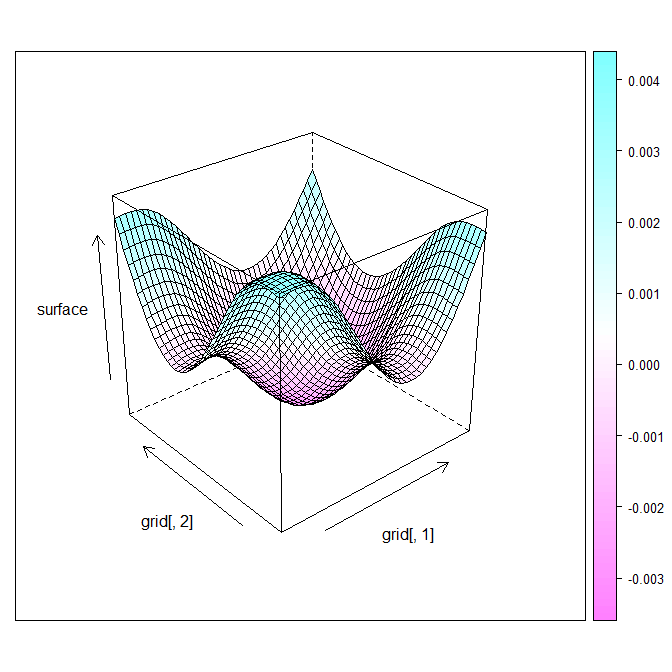
\includegraphics[width=.25\textwidth]{Images//basis_fn1.png}}
%\subfigure{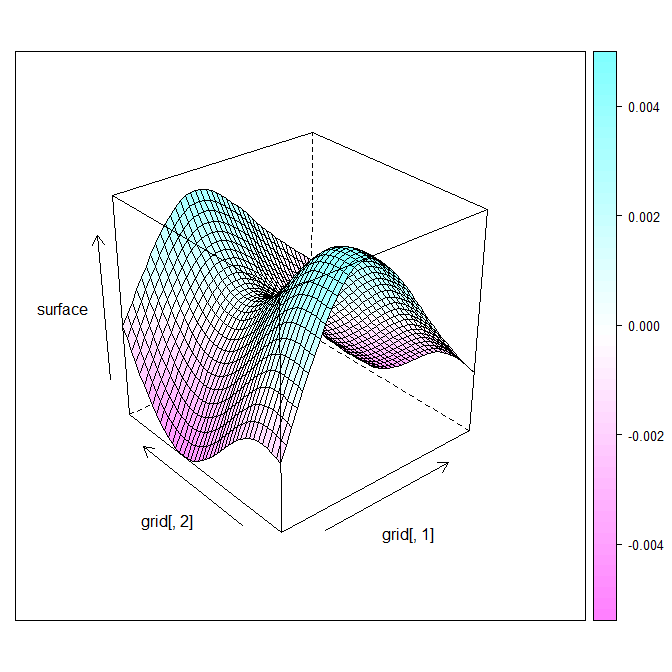
\includegraphics[width=.25\textwidth]{Images//basis_fn2.png}}
%\subfigure{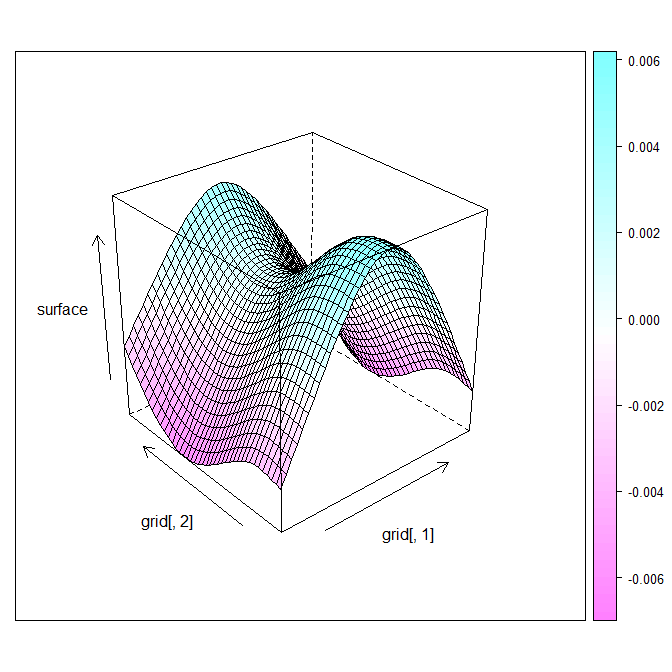
\includegraphics[width=.25\textwidth]{Images//basis_fn3.png}}
%\subfigure{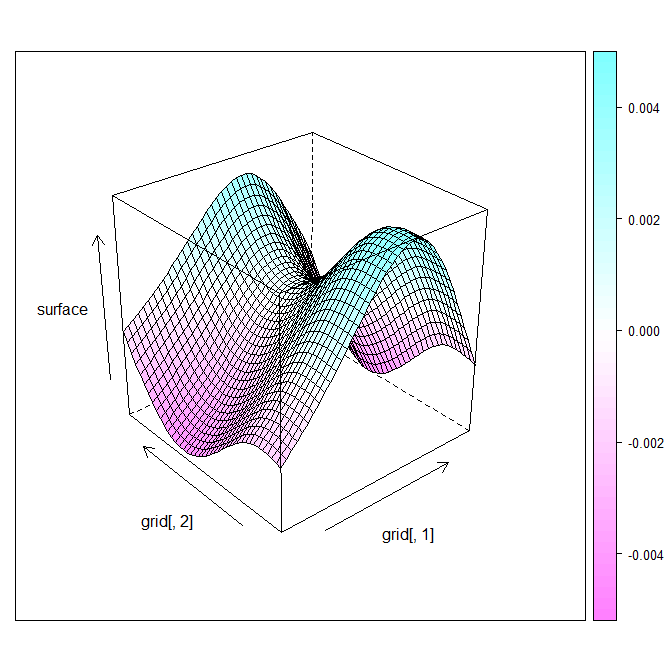
\includegraphics[width=.25\textwidth]{Images//basis_fn4.png}}
%\subfigure{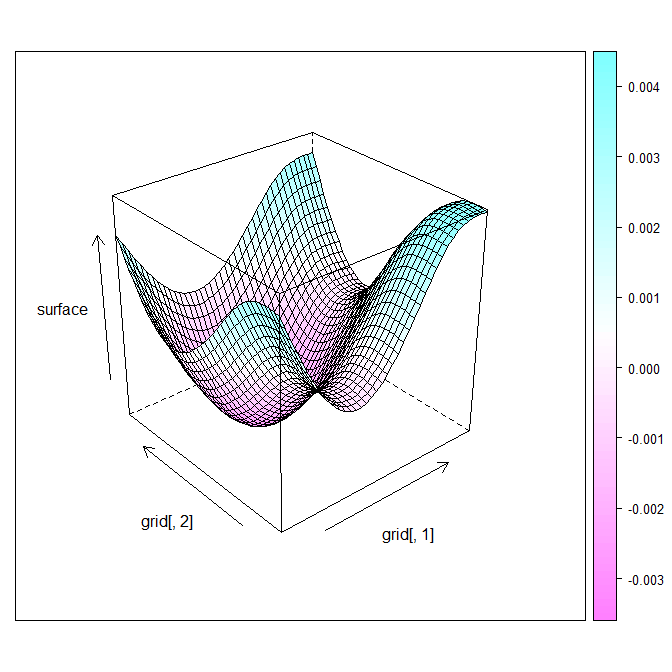
\includegraphics[width=.25\textwidth]{Images//basis_fn5.png}}
%\subfigure{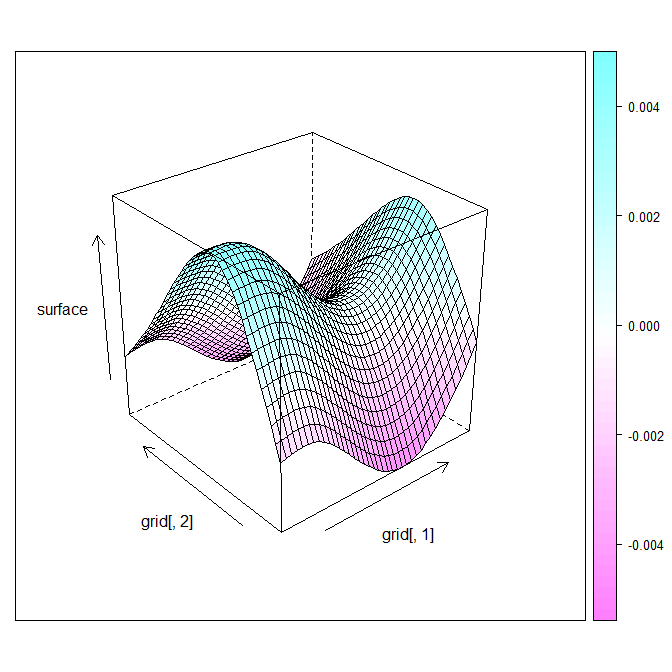
\includegraphics[width=.25\textwidth]{Images//basis_fn6.png}}
%\subfigure{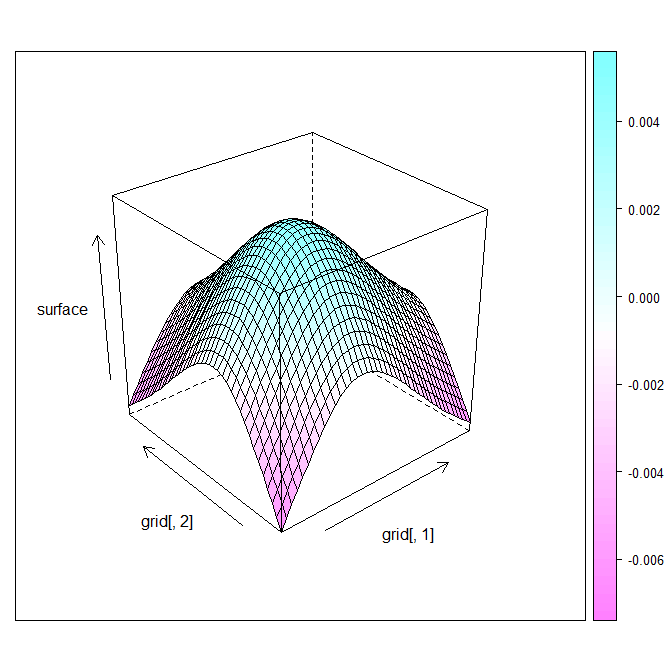
\includegraphics[width=.25\textwidth]{Images//basis_fn7.png}}
%\subfigure{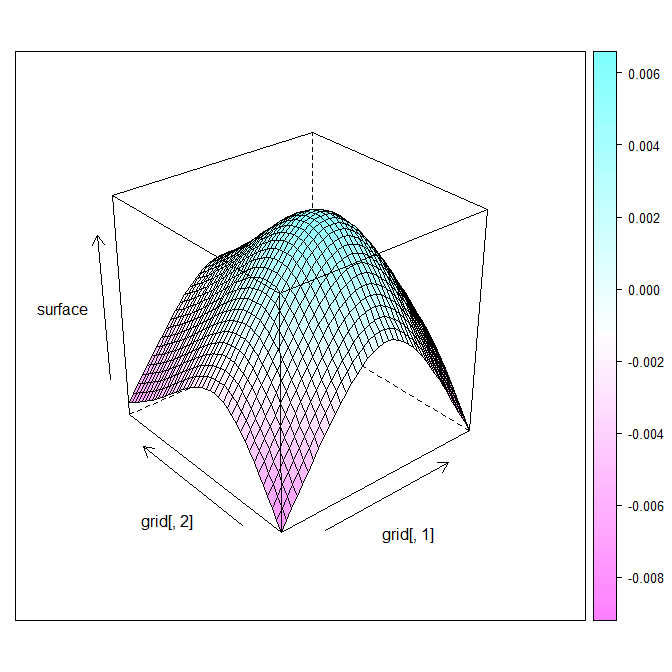
\includegraphics[width=.25\textwidth]{Images//basis_fn8.png}}
%\subfigure{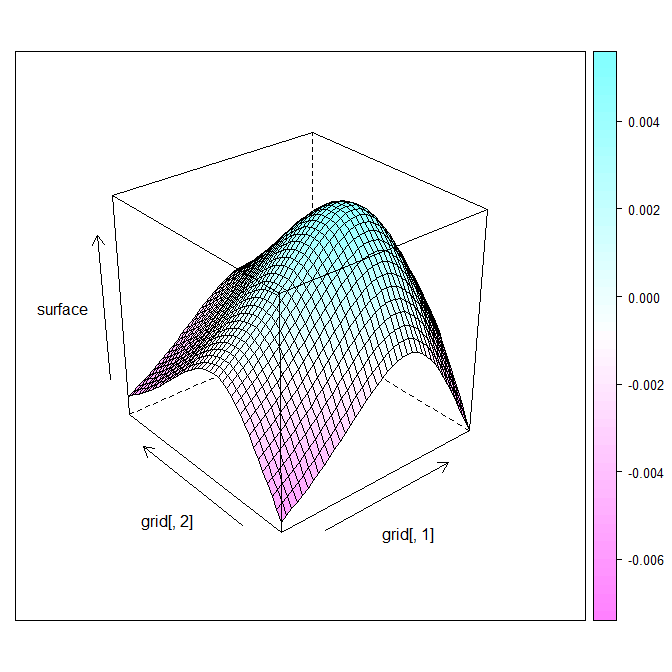
\includegraphics[width=.25\textwidth]{Images//basis_fn9.png}}
%\subfigure{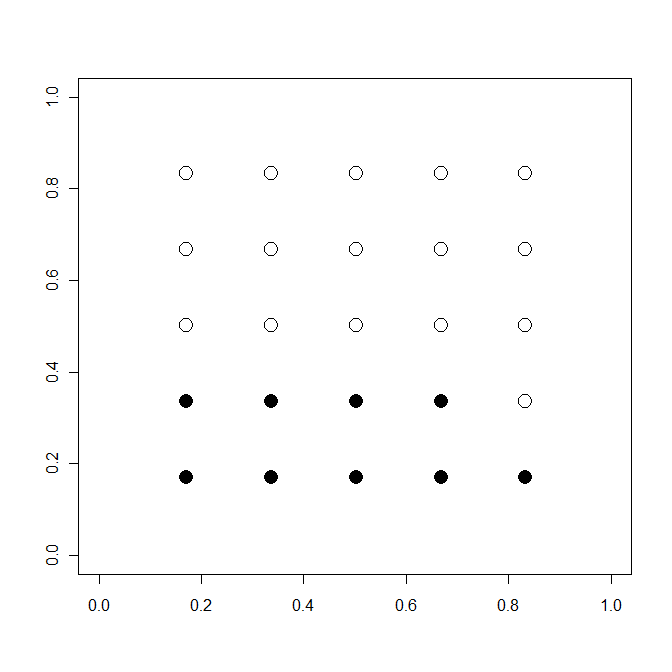
\includegraphics[width=.4\textwidth]{Images//knot_locations.png}}
%\caption{Plots of some of the basis functions in the penalized space. The plot on the bottom shows the corresponding knot location for each of the basis functions. The location of the black dot on the bottom left produced the basis function on the top left. The location of the black dot on the top right produced the basis function on the bottom right. }%
%\label{fig:basis_fns}%
%\end{figure}

%
%\begin{figure}%
%\centering
%\subfigure{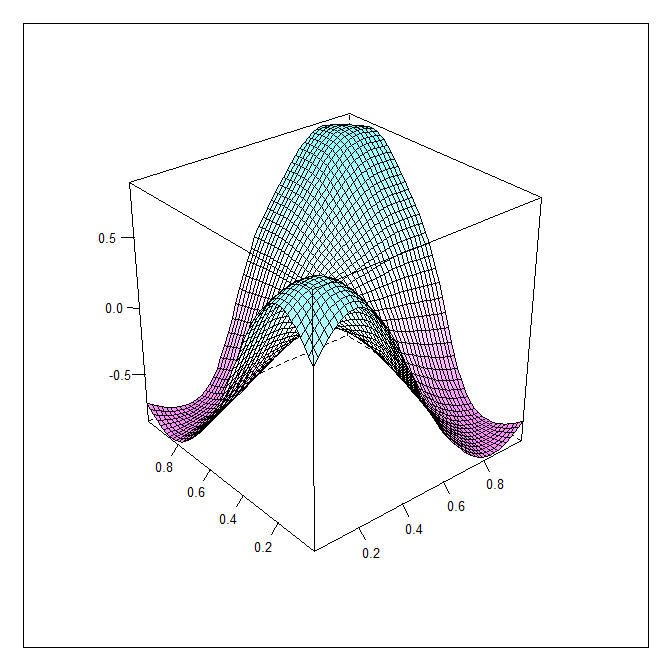
\includegraphics[width=.3\textwidth]{Images//est_cov.png}}
%\subfigure{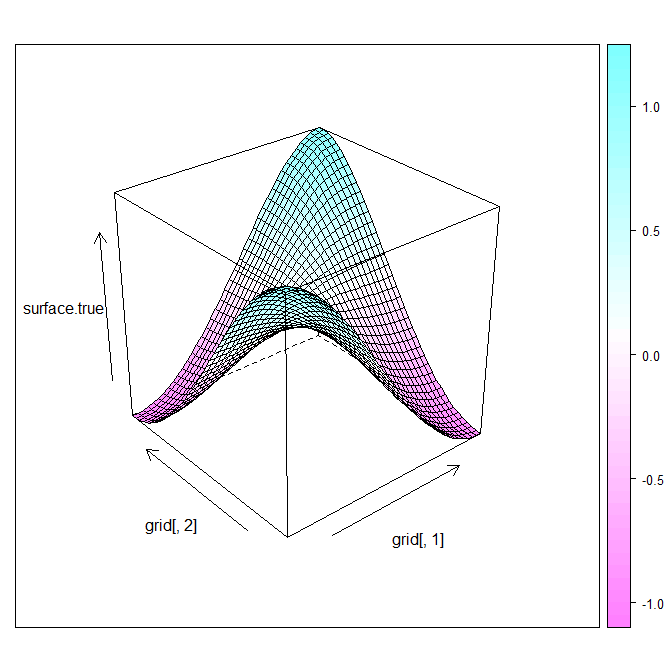
\includegraphics[width=.31\textwidth]{Images//true_cov.png}}
%\caption{Plot of estimated covariance function (left) and true covariance function (right). }%
%\label{fig:cov_est}%
%\end{figure}

%==========================================================
\section{Estimation of functional principal components } \label{eigenfunctions}
%==========================================================

Functional principal components are related to the well-known Karhunen-Loeve representation theorem.  For a square-integrable stochastic process $X(t)$ defined on a closed interval $[a,b]$,  with continuous covariance $C(s,t)$, there corresponds a linear operator $[T_Cf](s) = \int_a^bC(s,t)f(t)dt$. Since $C(s,t)$ is symmetric and non-negative definite, it has the following representation %(see Mercer's theorem)
\begin{equation*} 
 C(s,t) = \sum_{i=1}^{\infty}\lambda_i\psi_i(s)\psi_i(t),
\end{equation*}
where  $\{\psi_m(t)\}_{m=1,2,\ldots}$ are a sequence of orthonormal eigenfunctions which form a complete basis in $L_2[a,b]$, and  $\{\lambda_m \}_{m=1,2,\ldots}$ are nonnegative and nondecreasing eigenvalues. In this context, an eigenfunction-eigenvalue pair $\{\lambda_j, \psi_j(t)\}$ satisfy $\int_a^bC(s,t)\psi_j(t)dt = \lambda_j\psi_j(t)$. The Karhunen-Loeve theorem states that the process $X(t)$ admits the representation
\begin{equation*}
X(t) =  \sum_{m=1}^{\infty}\alpha_m \psi_m(t), \mbox{ where  } \alpha_m = \int_a^b X(t) \psi_m(t)dt,
\end{equation*}
and the random variables $\{\alpha_m \}_{m=1,2,\ldots}$ are uncorrelated and satisfy $E(\alpha_m)=0$ and Var($\alpha_m$) = $\lambda_m$, $\sum_m \lambda_m < \infty$. The eigenfunctions $\{\psi_m(t)\}_{m=1,2,\ldots}$ corresponding to $C(s,t)$ are called the principal component functions and the coefficients  $\{\alpha_m \}$ are the functional principal component scores of $X(t)$. We seek functions $\hat{\psi}(s)$ that satisfy satisfy
\begin{equation} \label{eq:eigenfuns}
\int \hat{C}(s,t)\hat{\psi}(t)dt=\theta\hat{\psi}(s).
\end{equation}

Methods for deriving principal component functions were developed in \cite{FDA} for functions represented by finite basis representation, i.e. $X(t) = \mathbf{b}'\mathbf{g}(t)$, where $\mathbf{g}(t)$ is a vector of basis functions. Using the finite dimensional covariance function representation in \eqref{eq:covest} we adapt these results by considering the vector of functions 
\begin{equation}
\mathbf{g(\cdot)}=(1, k_1(\cdot),R_{1}(\cdot, t_1),R_{1}(\cdot, t_2),\dots, R_{1}(\cdot, t_K))'.
\label{eq:g}
\end{equation}
Using $\mathbf{g}$ in \eqref{eq:g} the covariance function estimator in \eqref{eq:covest} has the representation $\hat{C}(s,t)= \mathbf{g}(s)'A\mathbf{g}(t)$ where
\vspace{0.8cm}
\begin{center}
 $A = \left(\begin{array}{cc:cccc}
d_{00,00} & d_{01,00} & c_{1.} & c_{2.} & \dots & c_{K.}\\
d_{00,01} & d_{01,01} & \sum_j c_{1j}k_1(t_j) & \sum_j c_{2j}k_1(t_j) & \dots & \sum_j c_{Kj}k_1(t_j)\\
\hdashline
c_{.1}   & \sum_j c_{j1}k_1(t_j) & c_{11}   & c_{12}   & \dots & c_{1K}\\
c_{.2}   & \sum_j c_{j2}k_1(t_j) & c_{21}   & c_{22}   & \dots & c_{2K}\\
\vdots  & \vdots                            & \vdots    & \vdots & \ddots    & \vdots \\
c_{.K}   & \sum_j c_{jK}k_1(t_j) & c_{K1}   & c_{K2}   & \dots & c_{KK}
\end{array}\right)$.
\end{center}
\vspace{0.8cm}
Note that  \cite{Cai:2010vr} use the tensor product norm on $\H\tprod \H$, thus there is no unpenalized subspace. In this case the matrix $A$ reduces to the bottom right submatrix. 
%Software packages, such as the gss package in R, will return the fitted coefficients $c$ and $d$ in \eqref{eq:covets}, The matrix $A$ can be constructed directly from the fitted coefficients in the output of the sspreg1() function which makes this straight forward to implement. 

Define the matrix $Q$ to be
\begin{equation*}
	Q_{ij} = \int_0^1\mathbf{g_i}(t)\mathbf{g}_j(t)dt,
\end{equation*}
then the following result states that the eigenfunctions can be expressed as a linear combination of the elements of $\mathbf{g}$.
\begin{lemma} \label{thm:eigenfunctions}
	The eigenfunctions of $\hat{C}(s,t)$ can be expressed as
	\begin{equation*}
		\hat{\psi}_k(\cdot) = \mathbf{b}'_k\mathbf{g}(\cdot),	
	\end{equation*}
	where $b_k$ is the $k$-th column of $B=Q^{-1/2}U$ and $U$ is the eigenvectors of $Q^{1/2}AQ^{1/2}$, and 
\[
\mathbf{g(\cdot)}=(1, k_1(\cdot),R_{1}(\cdot, t_1),R_{1}(\cdot, t_2),\dots, R_{1}(\cdot, t_K))'.
\]
\end{lemma}


%The intuition for the proof of Lemma \ref{thm:eigenfunctions} is more apparent when assuming from the start that the eigenfunctions have a finite basis expansion (see \cite{FDA}). 
%
%Suppose the function $\psi(\cdot)$ has representation  $\psi(s)=\mathbf{g}(s)'\mathbf{b}$. Substituting this expression into \eqref{eq:eigenfuns} we get
%\begin{equation}
%\int\mathbf{g}(s)'A\mathbf{g}(t)\mathbf{g}(t)'\mathbf{b}dt=\theta\mathbf{g}(s)'\mathbf{b}.
%\label{eq:cov_operator}
%\end{equation}
%
% Define symmetric matrix $Q=\int\mathbf{g'g}$, then equation (\ref{eq:cov_operator}) becomes
%\[
%\mathbf{g}(s)'AQ\mathbf{b}=\theta\mathbf{g}(s)'\mathbf{b},
%\]
%and since this equation must hold for all $s,$ this reduces to the
%following matrix equation
%\[
%AQ\mathbf{b}=\theta \mathbf{b}.
%\]
%Define the vector $\mathbf{u}=Q^{1/2}\mathbf{b},$ and hence $\mathbf{b}=Q^{-1/2}\mathbf{u}.$
%The solutions $\mathbf{b}$ to this eigen vector problem can be found
%by solving the equivalent symmetric eigenvector problem for $u,$
%\[
%Q^{1/2}AQ^{1/2}\mathbf{u}=\theta\mathbf{u}
%\]
% and setting $\mathbf{b}=Q^{-1/2}\mathbf{u}.$



%==========================================================
\section{Simulations }
%==========================================================

This section compares the finite sample performance of the FPC estimator to the finite basis expansion approach described in \cite{FDA}. The choice of smoothing individual curves or performing bivariate smoothing of the sample covariance is typically determined by the sparsity of observations on each curve. Generally one would smooth individual curves when they are densely observed, but smooth the sample covariance when curves are sparsely observed and presumably do not contain enough information at the individual curve level to capture all important features. From here on we will refer to bivariate smoothing of the covariance described in the paper as SSCOV and smoothing individual curves through finite basis expansions as SIC. The \texttt{pca.fd()} function in the R package  \texttt{fad} was used for the SIC method.

We compare these two approaches and focus is on the sparsity of data at the curve level by considering cases where the number of observations on each curve is equal to $m=5$, $m=10$, and $m=20$. We also consider a missing data case by removing a sequence of five observations from each curve in the data set where $m=20$. The resulting data sets have $m = 15$ observations per curve, and although the data are not missing at random the location along each curve where the five observations are missing is chosen at random for each curve. This type of missing data is common in remote sensing studies when a sensor runs out of battery power or malfunctions and has to be repaired or replaced, leaving a gap in the recorded data.

Random curves are simulated independently as
\begin{equation}
X(t) = \sum^{50}_{k=1}\zeta_k U_k \cos(k\pi t), \hspace{0.5cm} t \in [0,1],
\label{eq:sim process}
\end{equation}�
where $U_k$ were independently sampled from a Unif$(-\sqrt{3},\sqrt{3})$ distribution and \(\zeta=(-1)^{k+1}k^{-2}\). 
The covariance function for this process can be shown to be
\begin{equation*}
C(s,t) = \sum^{50}_{k=1}k^{-4} \cos(k\pi s)\cos(k\pi t). 
\end{equation*}�
As an illustration, the fitted covariance function for a single simulated data set is shown in Figure \ref{fig:covfits}.
%
%\begin{figure}
%        \centering
%        \begin{subfigure}[b]{0.24\textwidth}
%                \centering
%                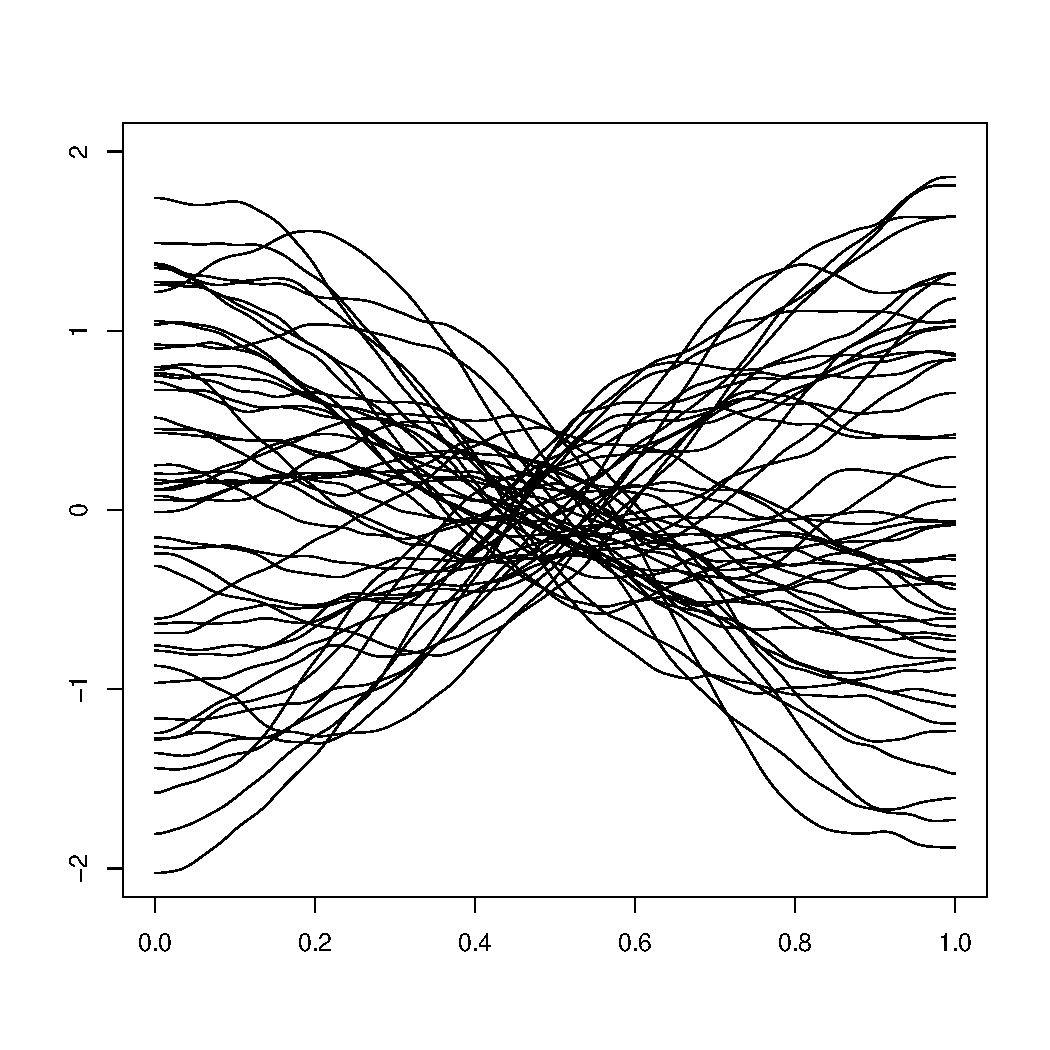
\includegraphics[width=\textwidth]{Images-nonparametric/cy-curves.pdf}
%                \caption{}
%        \end{subfigure}
%         \begin{subfigure}[b]{0.24\textwidth}
%                \centering
%                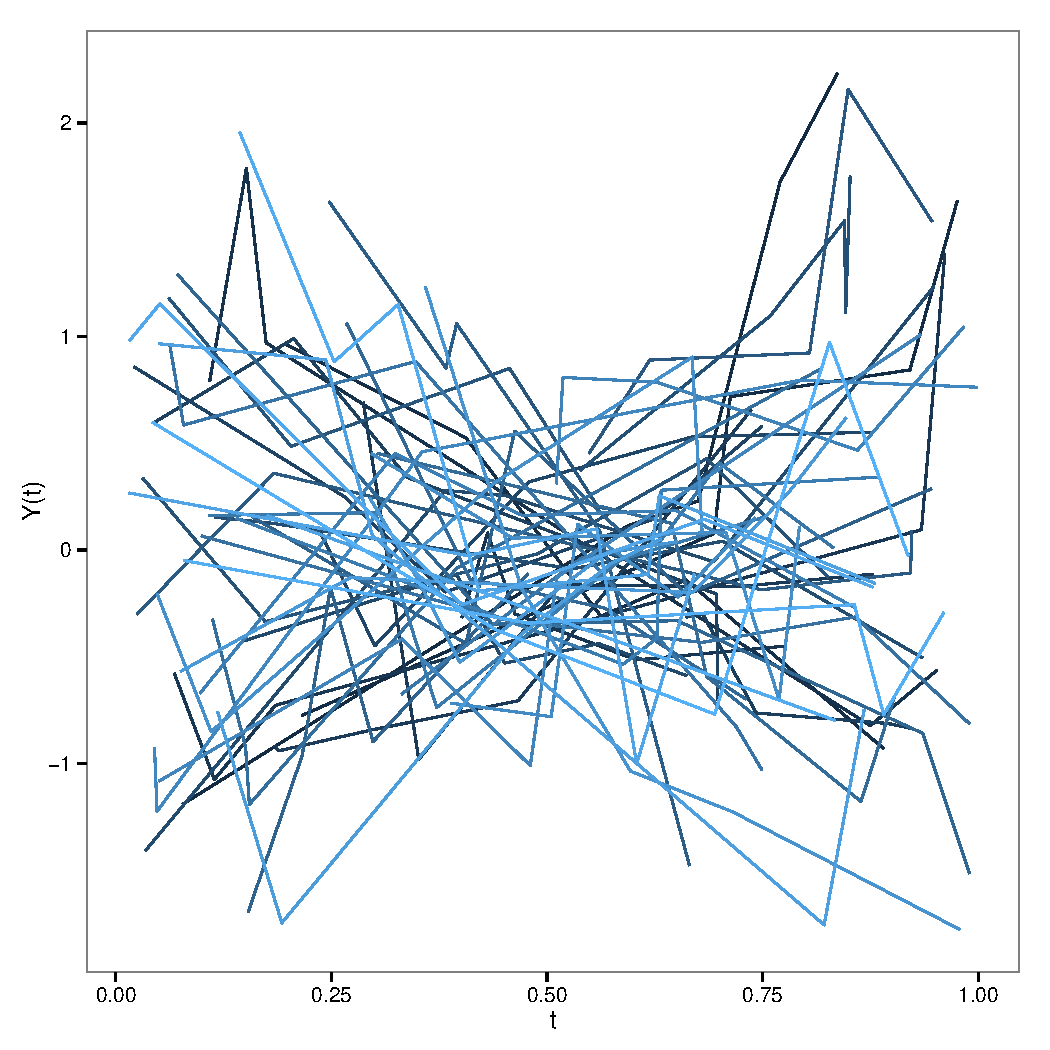
\includegraphics[width=\textwidth]{Images-nonparametric/cy-data-m5.pdf}
%                \caption{}
%                \label{}
%        \end{subfigure}
%        \begin{subfigure}[b]{0.24\textwidth}
%                \centering
%                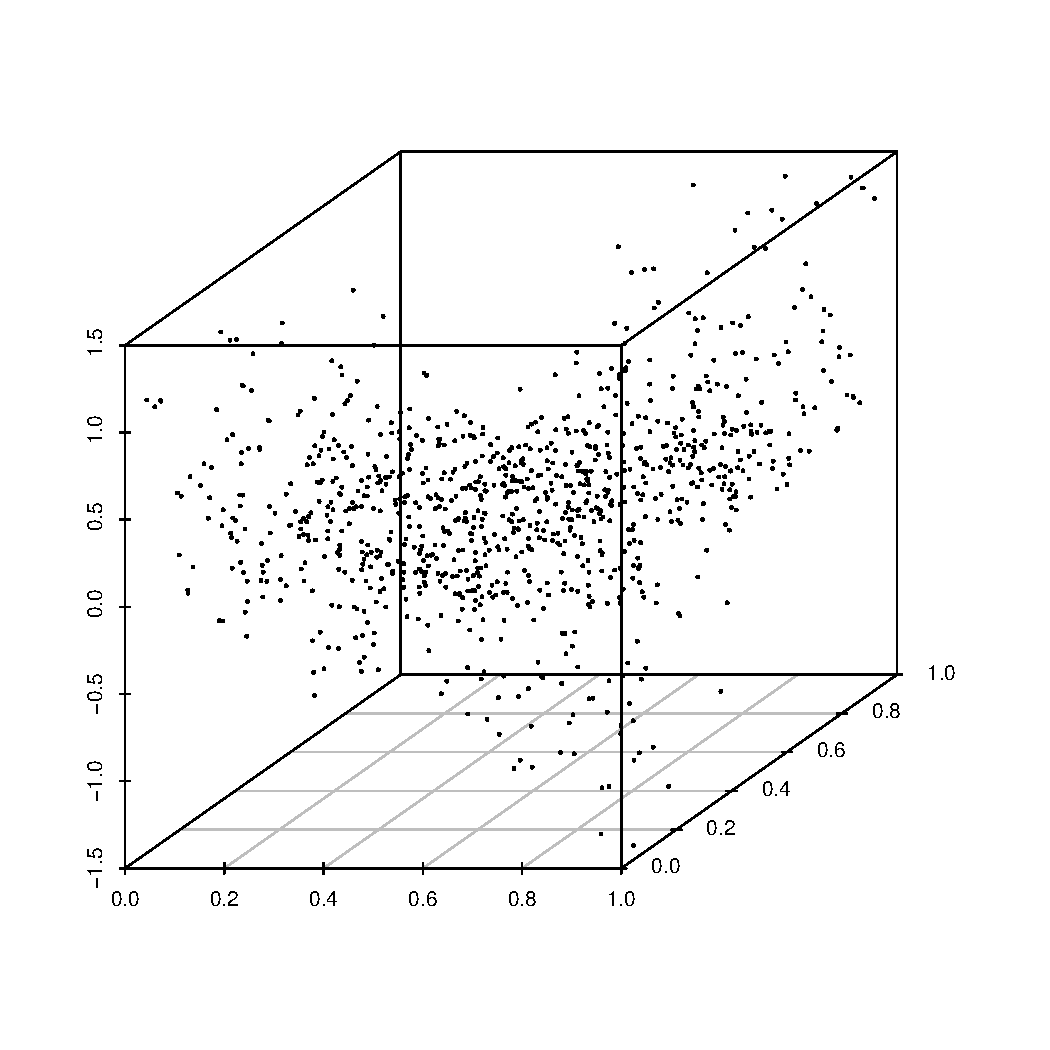
\includegraphics[width=\textwidth]{Images-nonparametric/cy-scatter3d-m5.pdf}
%                \caption{}
%                \label{}
%        \end{subfigure}% 
%          \begin{subfigure}[b]{0.24\textwidth}
%                \centering
%                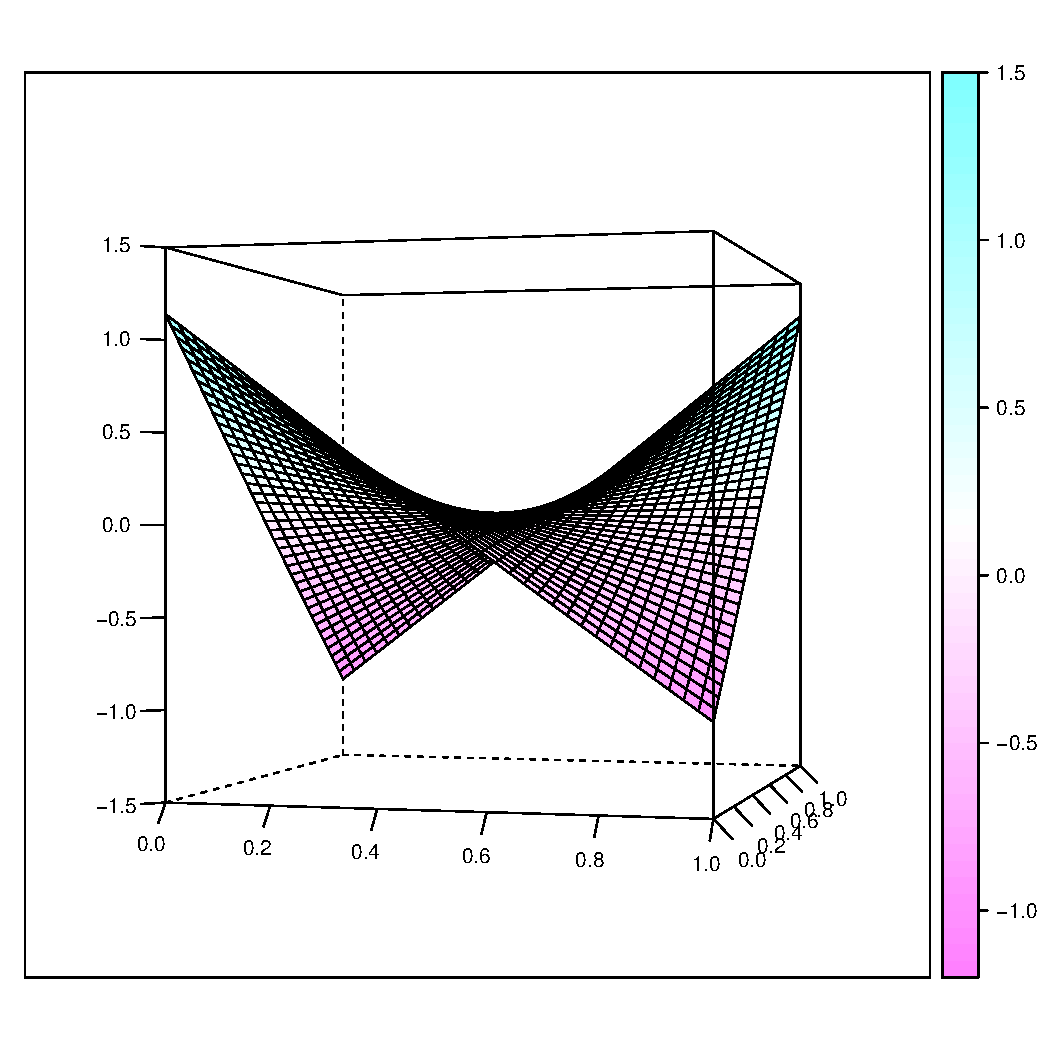
\includegraphics[width=\textwidth]{Images-nonparametric/cy-fit-wireframe-m5.pdf}
%                \caption{}
%                \label{}
%        \end{subfigure}% 
%        \caption{(a) 50 simulated curves from the process $X(t)$ in \eqref{eq:sim process} (b) data set of curves evaluated at five random locations with noise, $\sigma_0=0.392$ (c) Scatterplot of values based on the data used to estimate covariance surface (d) Estimated covariance function. }
%        \label{fig:sim curves}
% \end{figure}
 
 \begin{figure}
 	\centering   
        \begin{subfigure}[b]{0.40\textwidth}
                \centering
                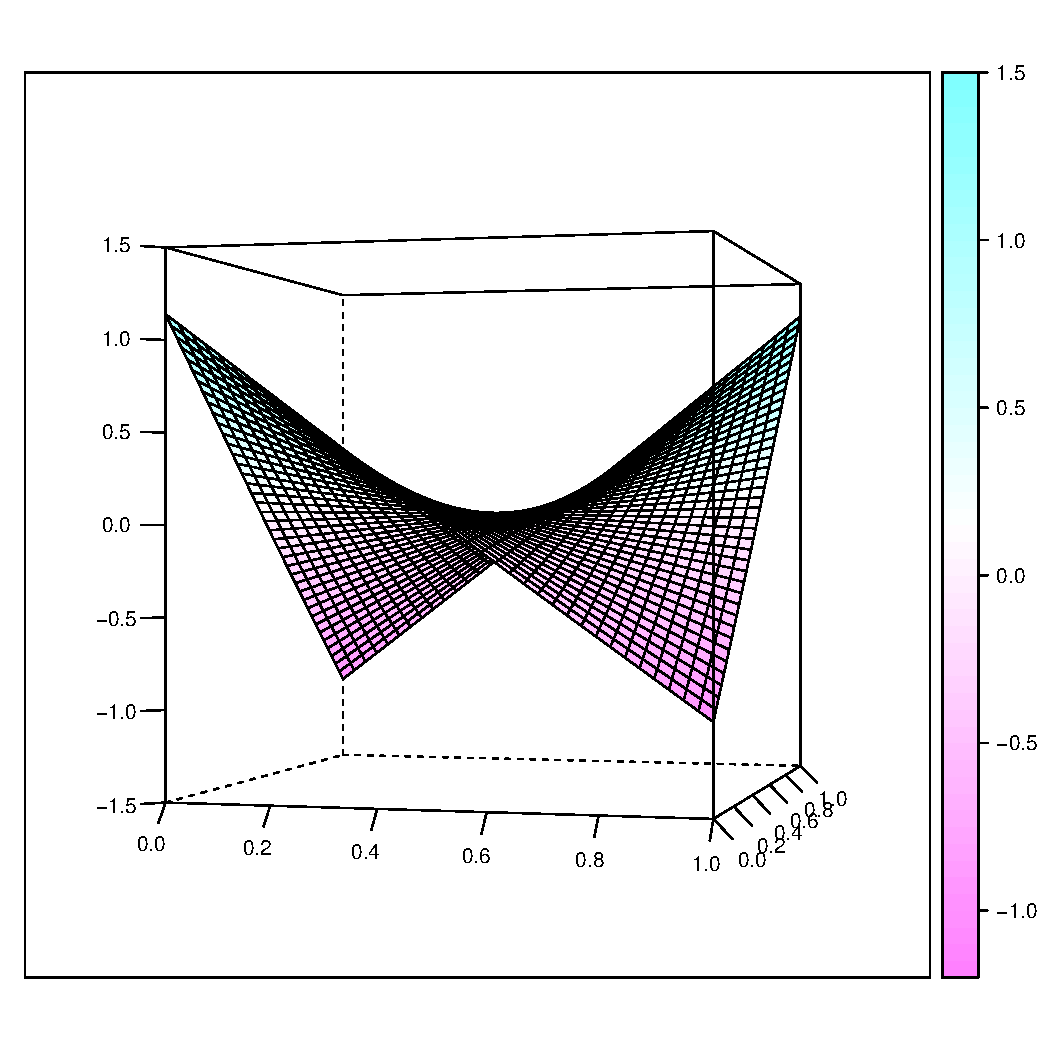
\includegraphics[width=\textwidth]{Images-nonparametric/cy-fit-wireframe-m5.pdf}
                \caption{m = 5}
                \label{}
        \end{subfigure}%
        \begin{subfigure}[b]{0.40\textwidth}
                \centering
                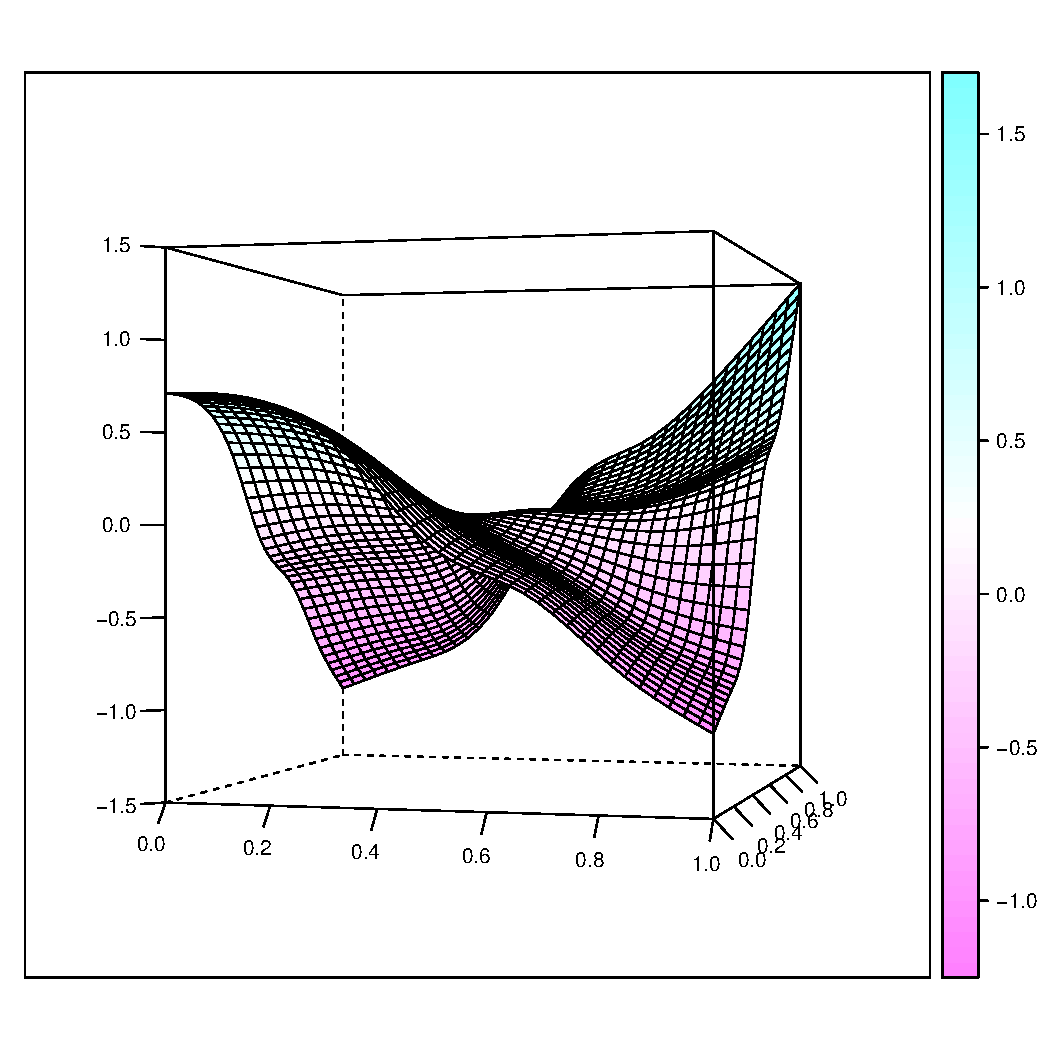
\includegraphics[width=\textwidth]{Images-nonparametric/cy-fit-wireframe-m10.pdf}
                \caption{m = 10}
                \label{}
        \end{subfigure}

        \begin{subfigure}[b]{0.40\textwidth}
                \centering
                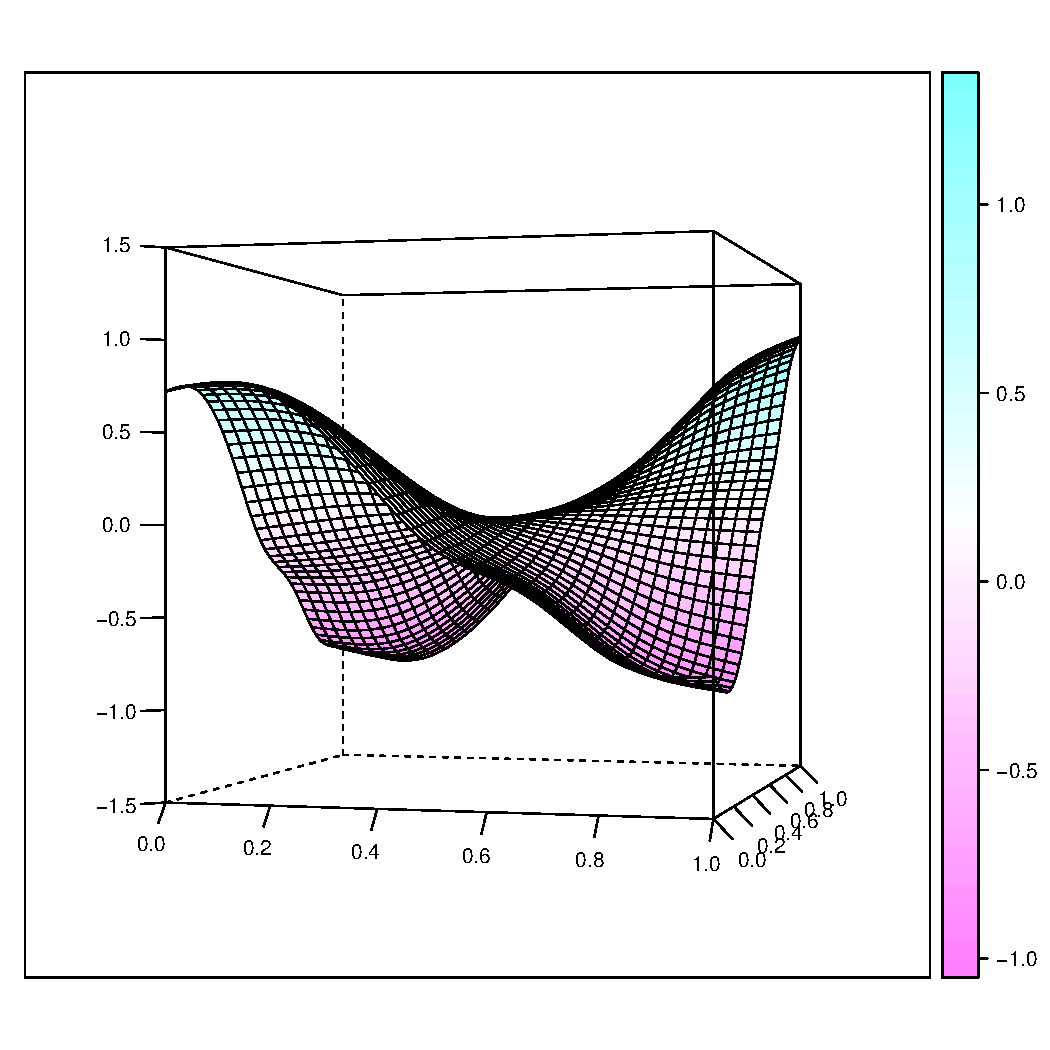
\includegraphics[width=\textwidth]{Images-nonparametric/cy-fit-wireframe-m40.pdf}
                \caption{m = 20}
                \label{}
        \end{subfigure}
                \begin{subfigure}[b]{0.40\textwidth}
                \centering
                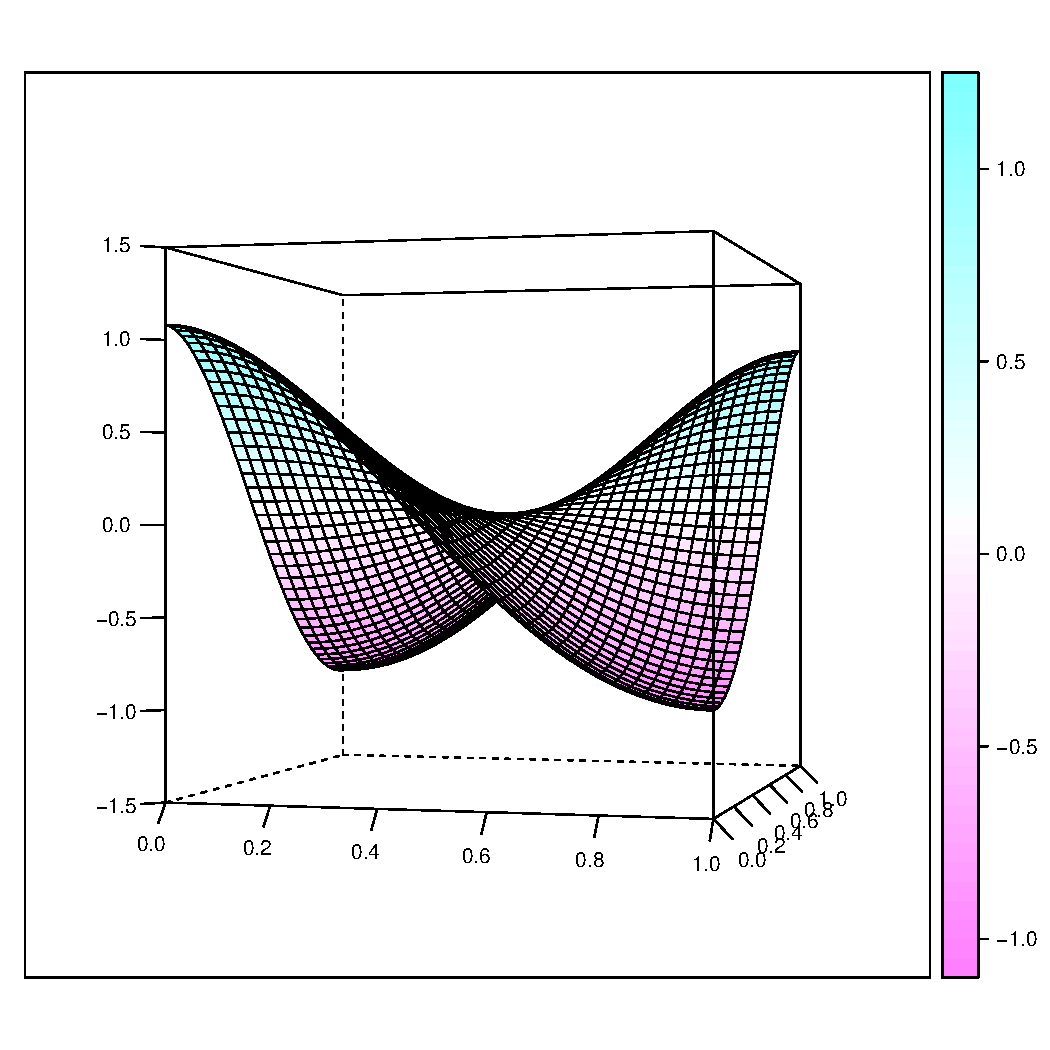
\includegraphics[width=\textwidth]{Images-nonparametric/cy-true-wireframe.pdf}
                \caption{truth}
                \label{}
        \end{subfigure}
        \caption{Estimated covariance functions using the SSCOV method an a data set consisting of 100 curves simulated from the process $X(t)$ in \eqref{eq:sim process} using observation standard deviation equal to $\sigma_0 = 0.329$. Here $m$ equals the number of observations for each curve. }
        \label{fig:covfits}
\end{figure}

To understand the general performance of the FPC estimator, we repeated this process 100 times using 100 curves with $\sigma_0=0.369$. Figures \ref{fig:fpca-ss} and \ref{fig:fpca-fda} show the pointwise mean and pointwise central 95\% quantile of the first two estimated functional principal components. Estimation error measured by integrated square error is summarized in Table \ref{tab:fpc-norm}. 

\begin{table}[ht]
\caption{Average integrated squared error $\norm{\hat{\psi}(t) - \psi(t)}^2_{L_2}$: averaged over 100 runs. The Monte Carlo standard error is shown in parentheses.}
\centering
\begin{tabular}{|c|l|cc|}
  \hline
 FPC & \# obs. per curve & SSCOV & SIC \\ 
  \hline
&  5  & 0.0231  (0.0018) & 0.0150  (0.0011) \\ 
 1st&  10 & 0.0142  (0.0009) & 0.0059 (0.0003) \\ 
 &  20 & 0.0064 (0.0005) & 0.0024  (0.0002) \\ 
 &  20 (5 missing) & 0.0098 (0.0007) & 0.0158 (0.0010) \\
   \hline
& 5 & 0.9750  (0.0727) & 0.8112  (0.0316) \\ 
 2nd & 10 & 0.4861 (0.0529) & 0.1401  (0.0110) \\ 
  &  20& 0.1148  (0.0113) & 0.0408  (0.0028) \\ 
  & 20 (5 missing) & 0.3826 (0.0476) & 0.4750 (0.0260) \\
   \hline
\end{tabular}
\label{tab:fpc-norm}
\end{table}

\begin{figure}
\begin{center}
\begin{tabular}{ccc}
  $m$ = 5 & $m$ = 10 & $m$ = 20  \\
   \includegraphics[width=2in]{Images-nonparametric/sim-study/fpc1-fpca-ss-params-ind-5.pdf} &
      \includegraphics[width=2in]{Images-nonparametric/sim-study/fpc1-fpca-ss-params-ind-10.pdf} &
         \includegraphics[width=2in]{Images-nonparametric/sim-study/fpc1-fpca-ss-params-ind-20.pdf} \\
      \includegraphics[width=2in]{Images-nonparametric/sim-study/fpc2-fpca-ss-params-ind-5.pdf} &
      \includegraphics[width=2in]{Images-nonparametric/sim-study/fpc2-fpca-ss-params-ind-10.pdf} &
         \includegraphics[width=2in]{Images-nonparametric/sim-study/fpc2-fpca-ss-params-ind-20.pdf} \\  
\end{tabular}
\end{center}
\caption{Functional principal component estimation using the SSCOV method. For each of the 100 simulated data sets 100 curves were simulated with $m$ observations per curve. The solid line is the pointwise mean, the dashed line is the true FPC, and the gray bands show the pointwise 2.5 and 97.5 quantiles.}
\label{fig:fpca-ss}
\end{figure}


\begin{figure}
\begin{center}
\begin{tabular}{ccc}
 $m$ = 5 & $m$ = 10 & $m$ = 20  \\
   \includegraphics[width=2in]{Images-nonparametric/sim-study/fpc1-fpca-fda-params-ind-5.pdf} &
      \includegraphics[width=2in]{Images-nonparametric/sim-study/fpc1-fpca-fda-params-ind-10.pdf} &
         \includegraphics[width=2in]{Images-nonparametric/sim-study/fpc1-fpca-fda-params-ind-20.pdf} \\
      \includegraphics[width=2in]{Images-nonparametric/sim-study/fpc2-fpca-fda-params-ind-5.pdf} &
      \includegraphics[width=2in]{Images-nonparametric/sim-study/fpc2-fpca-fda-params-ind-10.pdf} &
         \includegraphics[width=2in]{Images-nonparametric/sim-study/fpc2-fpca-fda-params-ind-20.pdf} \\  
\end{tabular}
\end{center}
\caption{Functional principal component estimation using the SIC method as described in \cite{FDA}. For each of the 100 simulated data sets 100 curves were simulated with $m$ observations per curve. The solid line is the pointwise mean, the dashed line is the true FPC, and the gray bands show the pointwise 2.5 and 97.5 quantiles.}
\label{fig:fpca-fda}
\end{figure}

\begin{figure}
\begin{center}
\begin{tabular}{cc}
SSCOV & SIC \\
   \includegraphics[width=2in]{Images-nonparametric/sim-study/fpc1-gap2-ss-20.pdf} &
         \includegraphics[width=2in]{Images-nonparametric/sim-study/fpc1-gap2-fda-20.pdf} \\
      \includegraphics[width=2in]{Images-nonparametric/sim-study/fpc2-gap2-ss-20.pdf} &
         \includegraphics[width=2in]{Images-nonparametric/sim-study/fpc2-gap2-fda-20.pdf} \\  
\end{tabular}
\end{center}
\caption{For each of the 100 simulated data sets 100 data were simulated with $20$ observations per curve, then for each curve a random sequence of five observations was removed to create a gap in the observation process. The solid line is the pointwise mean, the dashed line is the true FPC, and the gray bands show the pointwise 2.5 and 97.5 quantiles.}
\label{default}
\end{figure}

\section{Discussion} \label{ch2:discussion}

We have shown how the reproducing kernel Hilbert space framework for covariance estimation can be extended to allow the use of function spaces where the penalty functional induces a non-empty unpenalized subspace (Why would you want to do this for covariance function estimation??? I don't know, and I my current thinking is that you likely wouldn't want to do this). We have also derived the form of the principal component functions. Even though development here was for a specific penalty, the method is very general and could easily be applied to other penalties, though the form of the reproducing kernel and the basis for the null space will depend on this choice. 

Though the general wisdom is to avoid smoothing individual curves with sparse data, our simulations show that this approach  performs slightly better for our sparse case ($m = 5$) as well as the other cases we considered. This superior performance might be due to the fact that the curves we simulated are fairly smooth, hence even relatively few observations are enough to recover the main features. The only case where smoothing the covariance performed better was in our ``missing data'' scenario, where we removed a random gap of five observations (25\% of the data per curve). We believe this is a reasonable type of missing data as it can occur from malfunctioning sensors or sensors that experience a period without power. In this case loss of information at the curve level is large and pooling data is important in order to recover important features, as our simulations confirm. 

We have also created an R package implementation of this method with user-friendly functions for estimating the covariance function and principal component functions for functional data, making it convenient to use empirical basis representation for functional data analyses. Documentation for the R package is included in appendix. 



\section{Proofs} \label{ch2:proofs}
Proof of Lemma \ref{thm:eigenfunctions}
\begin{proof}
Let $\theta_k$ be the eigenvalues of $Q^{1/2}AQ^{1/2}$, then
\begin{align*}
	\sum \theta_k \hat{\psi}_k(s)\hat{\psi}_k(t) &= \sum \theta_kb'_k\mathbf{g}(s)b'_k\mathbf{g}(t) \\
							&= \sum \theta_k\mathbf{g}'(s)b_kb'_k\mathbf{g}(t) \\
							&= \mathbf{g}'(s)\left( B  \begin{bmatrix}
								\theta_1 &  &  &\\
								&  \ddots &\\
								&  & \theta_k
							      \end{bmatrix} B' \right) \mathbf{g}(t).
\end{align*}
To complete the proof, we show that $B  \begin{bmatrix}
								\theta_1 &  &  &\\
								&  \ddots &\\
								&  & \theta_k
							      \end{bmatrix} B'=A$,
\begin{align*}
	B \begin{bmatrix}
							\theta_1 &  &  &\\
								&  \ddots &\\
								&  & \theta_k
							      \end{bmatrix} B' &= Q^{-1/2}U  \begin{bmatrix}
								\theta_1 &  &  &\\
								&  \ddots &\\
								&  & \theta_k
							      \end{bmatrix} U'Q^{-1/2}\\
							     &= Q^{-1/2}[\theta_1\mathbf{u}_1| \dots  |\theta_k\mathbf{u}_k] U'Q^{-1/2}\\
							     &= Q^{-1/2}[Q^{1/2}AQ^{1/2}\mathbf{u}_1| \dots| Q^{1/2}AQ^{1/2}\mathbf{u}_k] U'Q^{-1/2}\\
							     &= Q^{-1/2}Q^{1/2}AQ^{1/2}U U'Q^{-1/2}\\
							     &= A. 
\end{align*}
Thus, $\sum \theta_k \hat{\psi}_k(s)\hat{\psi}_k(t) = g'(s)Ag(t) = \hat{C}(s,t)$. \qedhere
\end{proof}


%\begin{figure}[htbp]
%\begin{center}
%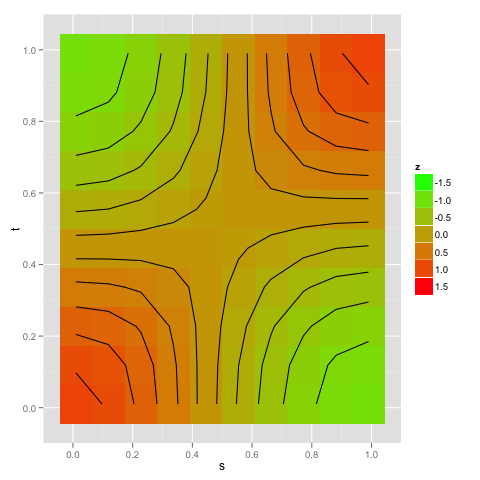
\includegraphics[width = 0.5\textwidth ]{images/Ch3/covfun.png}
%\caption{Covariance function}
%\label{default}
%\end{center}
%\end{figure}



%\begin{figure}[htbp]
%\begin{center}
%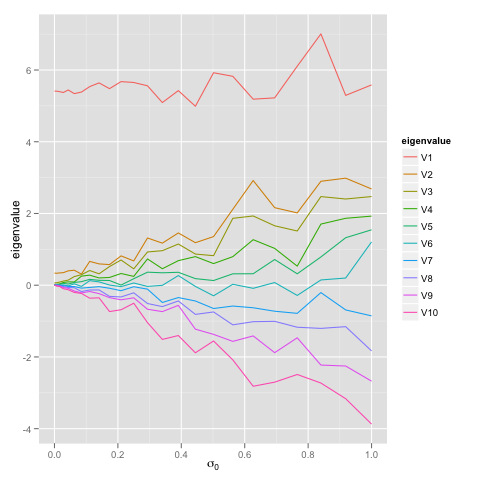
\includegraphics[width = 0.8\textwidth ]{images/Ch3/eval-seq.png}
%\caption{default}
%\label{default}
%\end{center}
%\end{figure}
%
%\begin{figure}[htbp]
%\begin{center}
%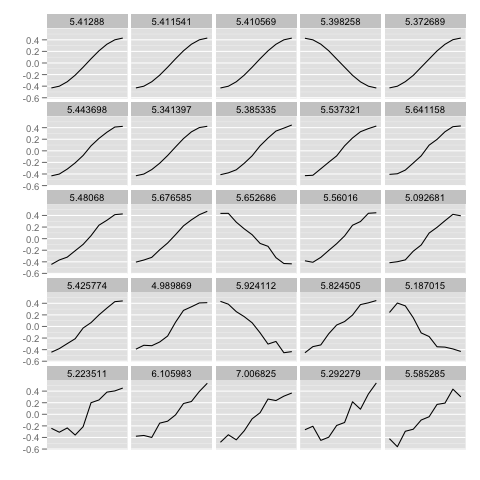
\includegraphics[width = 0.8\textwidth ]{images/Ch3/first-efun.png}
%\caption{default}
%\label{default}
%\end{center}
%\end{figure}
%
%\begin{figure}[htbp]
%\begin{center}
%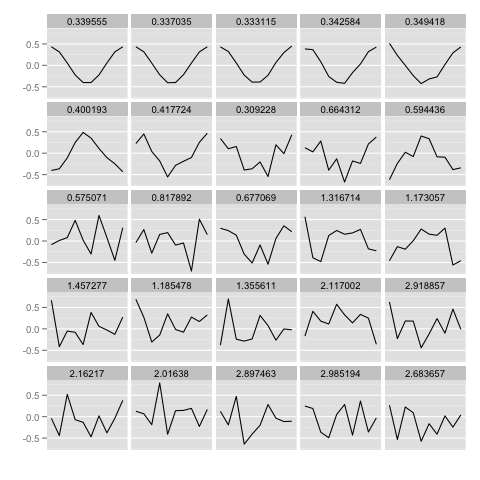
\includegraphics[width = 0.8\textwidth ]{images/Ch3/second-efun.png}
%\caption{default}
%\label{default}
%\end{center}
%\end{figure}




